\chapter{Theory}

\section{Sobel operator}
\label{Sobel}
The Sobel operator can be used to calculate the gradients in the image intensity...
Dynamic range and normalization...
Border handling...

\section{Accelerator design} 
\paragraph*{}
This section describes the design of the accelerator and explain how the pixel data is handled when travelling from external memory to the accelerator and back to external memory. 
Because each memory transaction involves two pixels (16bit data width). The proposed design of the accelerator, will process two pixels in parallel, this will increase the throughput without increasing the clock rate. At the same time it also simplifies the data handling, since the accelerator does not need to distinguish between which pixel to process (lower byte or upper byte). The drawback of this parallel approach is that the combinatorial logic that performs the Sobel operation, will be twice as big.

\paragraph*{}
As seen in the previous section \ref{Sobel}, any given pixel, in the output image of the Sobel operator, is a function of the surrounding eight pixels in the input image. This requires that the accelerator must have access to these surrounding pixels, in order to evaluate the Sobel operator. Instead of reading the entire neighborhood from the external RAM, for every single pixel, an obvious improvement is to use a sliding window technique, and thereby minimizing the number of memory transactions. If two pixel are to be processed in parallel, a 3x4 sliding window is required. But since the two convolution kernels stretches over three memory addresses the width of the sliding window must be increased by one pixel to a total of 3x5 pixels.
Figure \ref{fig:shift_register} shows the proposed sliding window and illustrates how incoming pixels are shifted from right to left.

\begin{figure}[H]
	\centering
	%\includegraphics[width=0.5 \textwidth]{shift_register.svg}
	\caption{Shift register}
	\label{fig:shift_register}
\end{figure}

A block diagram showing the internal architecture of the accelerator is seen in figure \ref{fig:AccBlockDiagram}. The figure shows how data will flow from memory, over the sliding window through the Sobel operator and back to the memory again. A few control signals to control the memory and sliding window are also depicted in the figure. 

\begin{figure}[H]
	\centering
	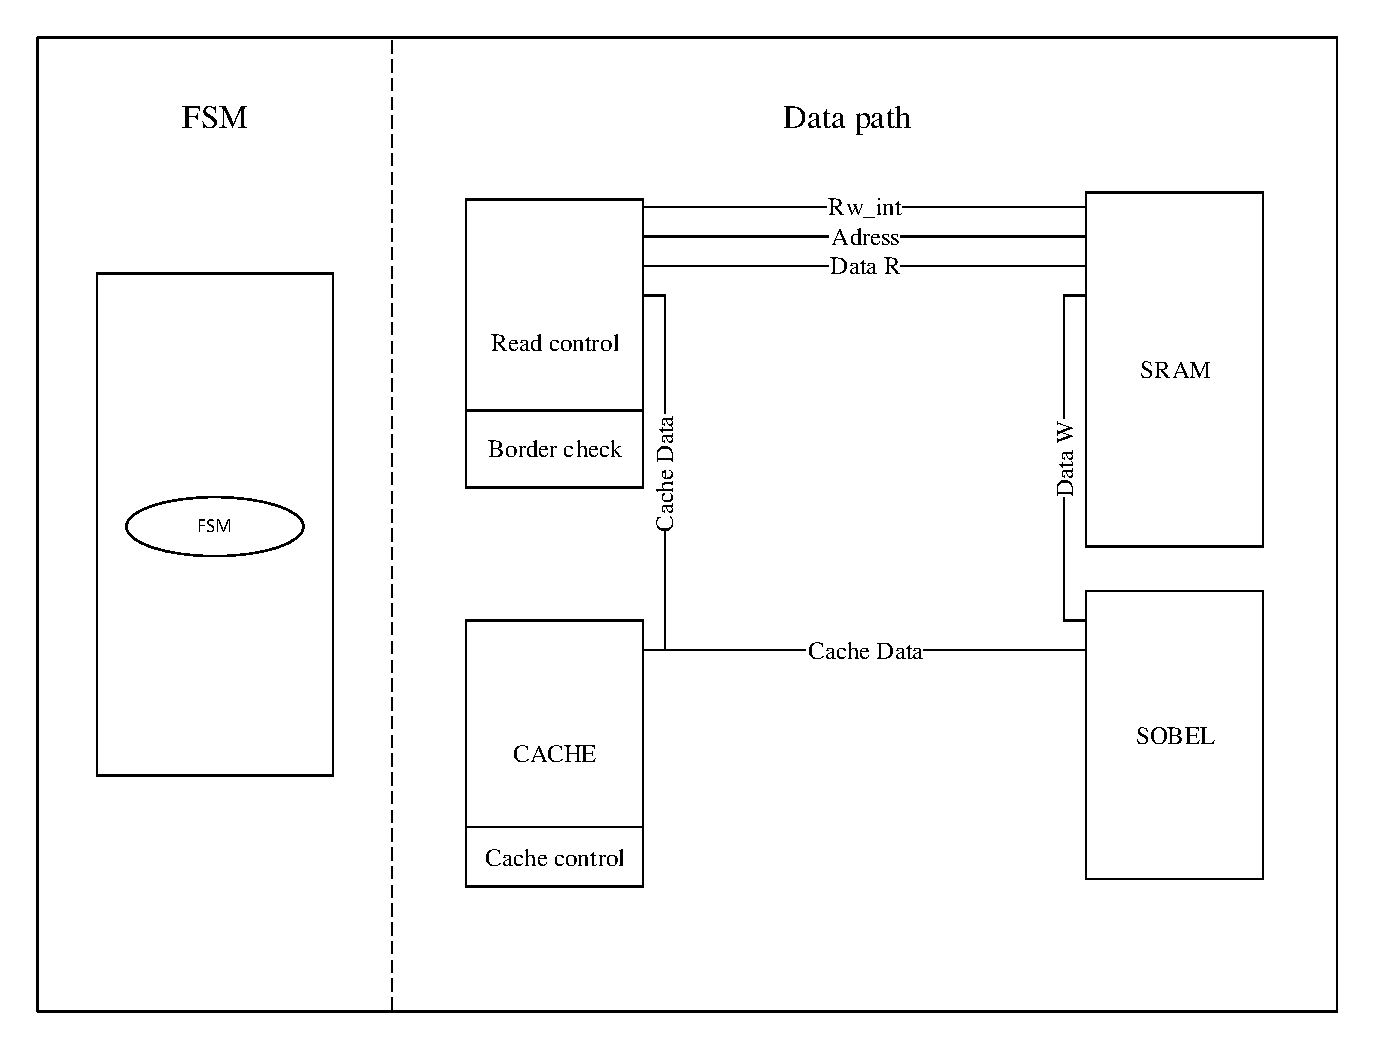
\includegraphics[width=1.0 \textwidth]{Block_diagram.pdf}
	\caption{Internal architecture of the accelerator}
	\label{fig:AccBlockDiagram}
\end{figure}

\paragraph*{}
From the architecture seen in figure \ref{fig:AccBlockDiagram} along with sliding window from figure \ref{fig:shift_register} it is possible to give an initial estimate of the attainable throughput of the accelerator. For each processed pixel pair, the accelerator is required to perform three memory reads and one memory write. Because the memory controller needs to setup the address prior to reading and writing, two extra cycles are to be expected, giving a total of six clock cycles per pixel pair.
With a clock frequency of 12.5 MHz (maximum when the memory is operated in asynchronous mode) this gives a throughput of approximately 4.1M pixel/sec.

\paragraph*{}
Figure \ref{fig:ASM_HW} shows a complete ASMD diagram of the proposed design. The ASMD diagram also covers details about such as border handling all states from start 

\begin{figure}[H]
	\centering
	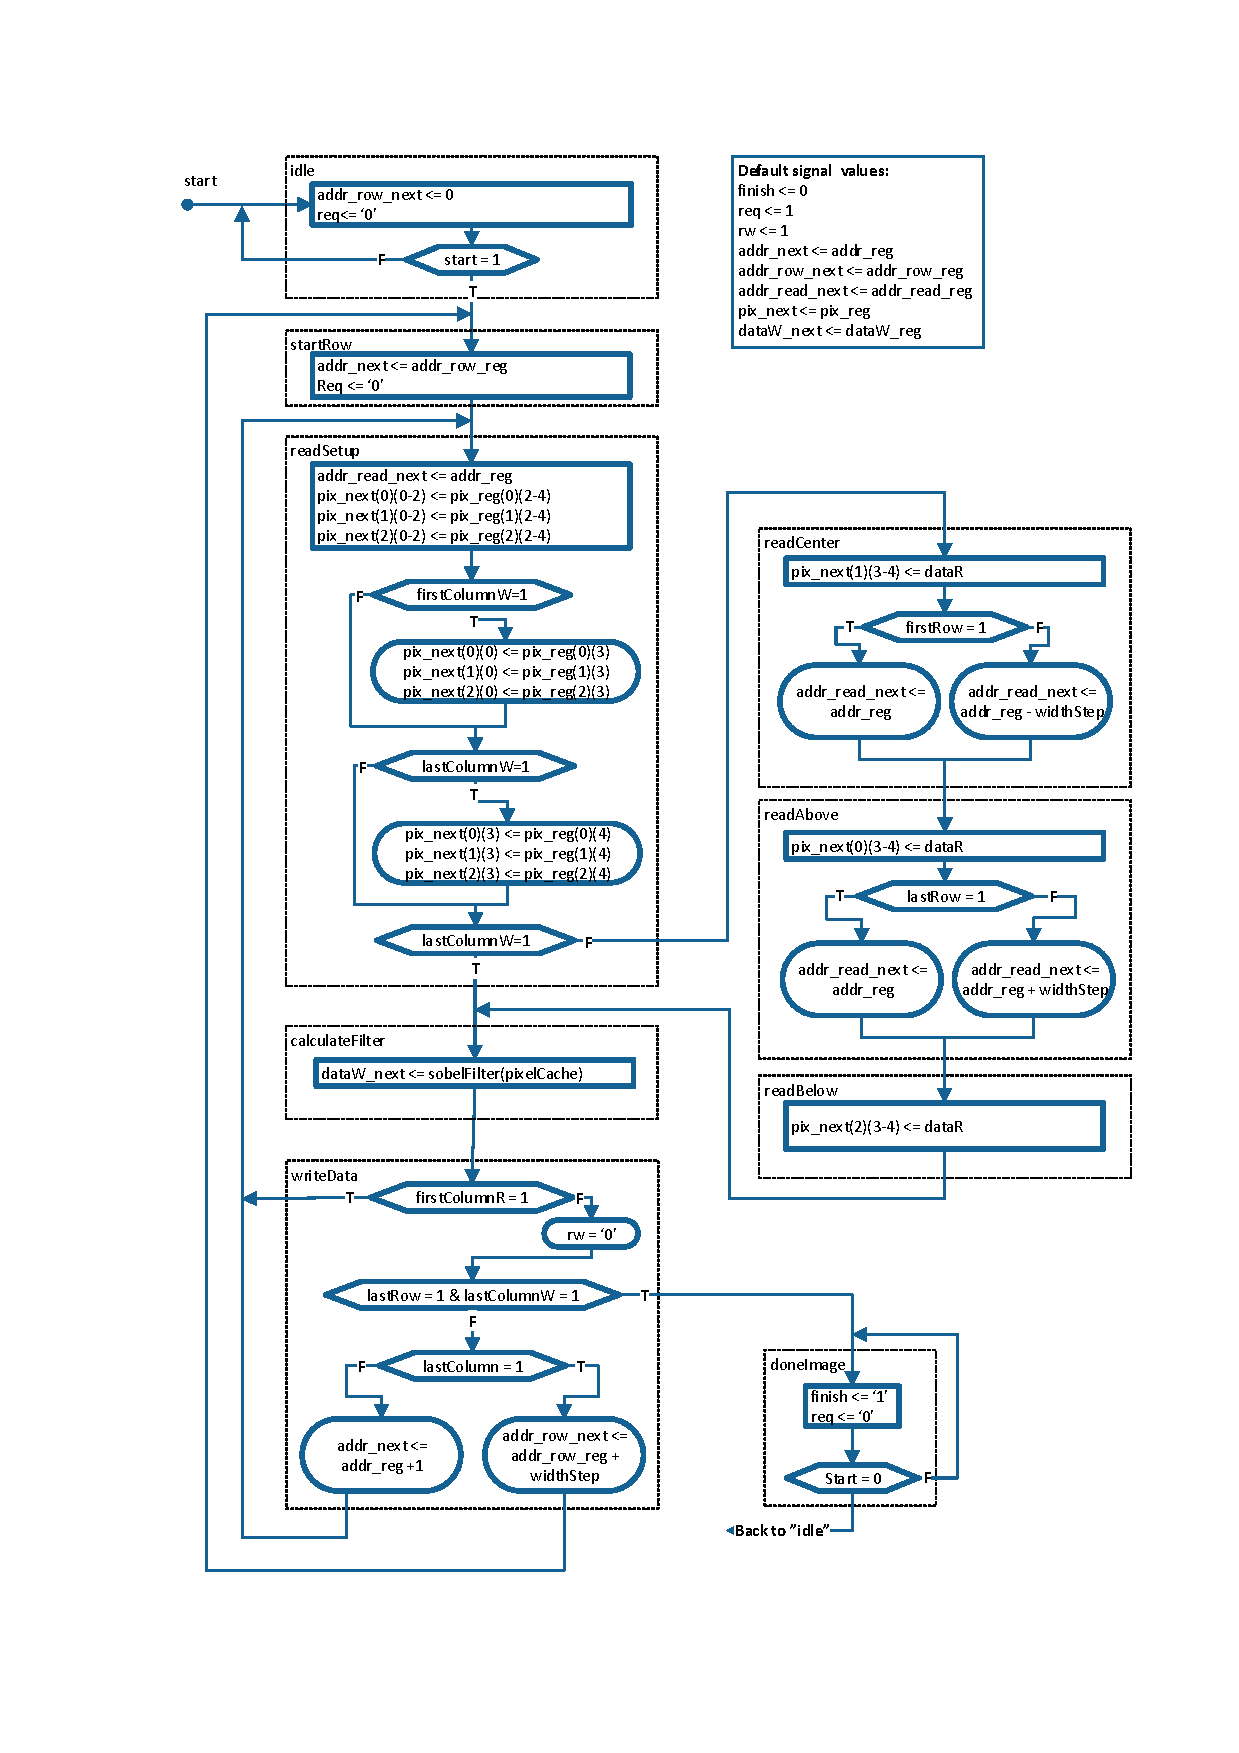
\includegraphics[width=1 \textwidth]{ASM_HWacc.pdf}
	\caption{ASMD chart for the edge detector hardware accelerator}
	\label{fig:ASM_HW}
\end{figure}

\section{HW}
\label{sec:hw}
PUT some text\\
put some cite \cite[p.11~eq.2.6]{Book}, \cite[p.11~eq.2.6]{Note}

\begin{figure}[H]
	\centering
	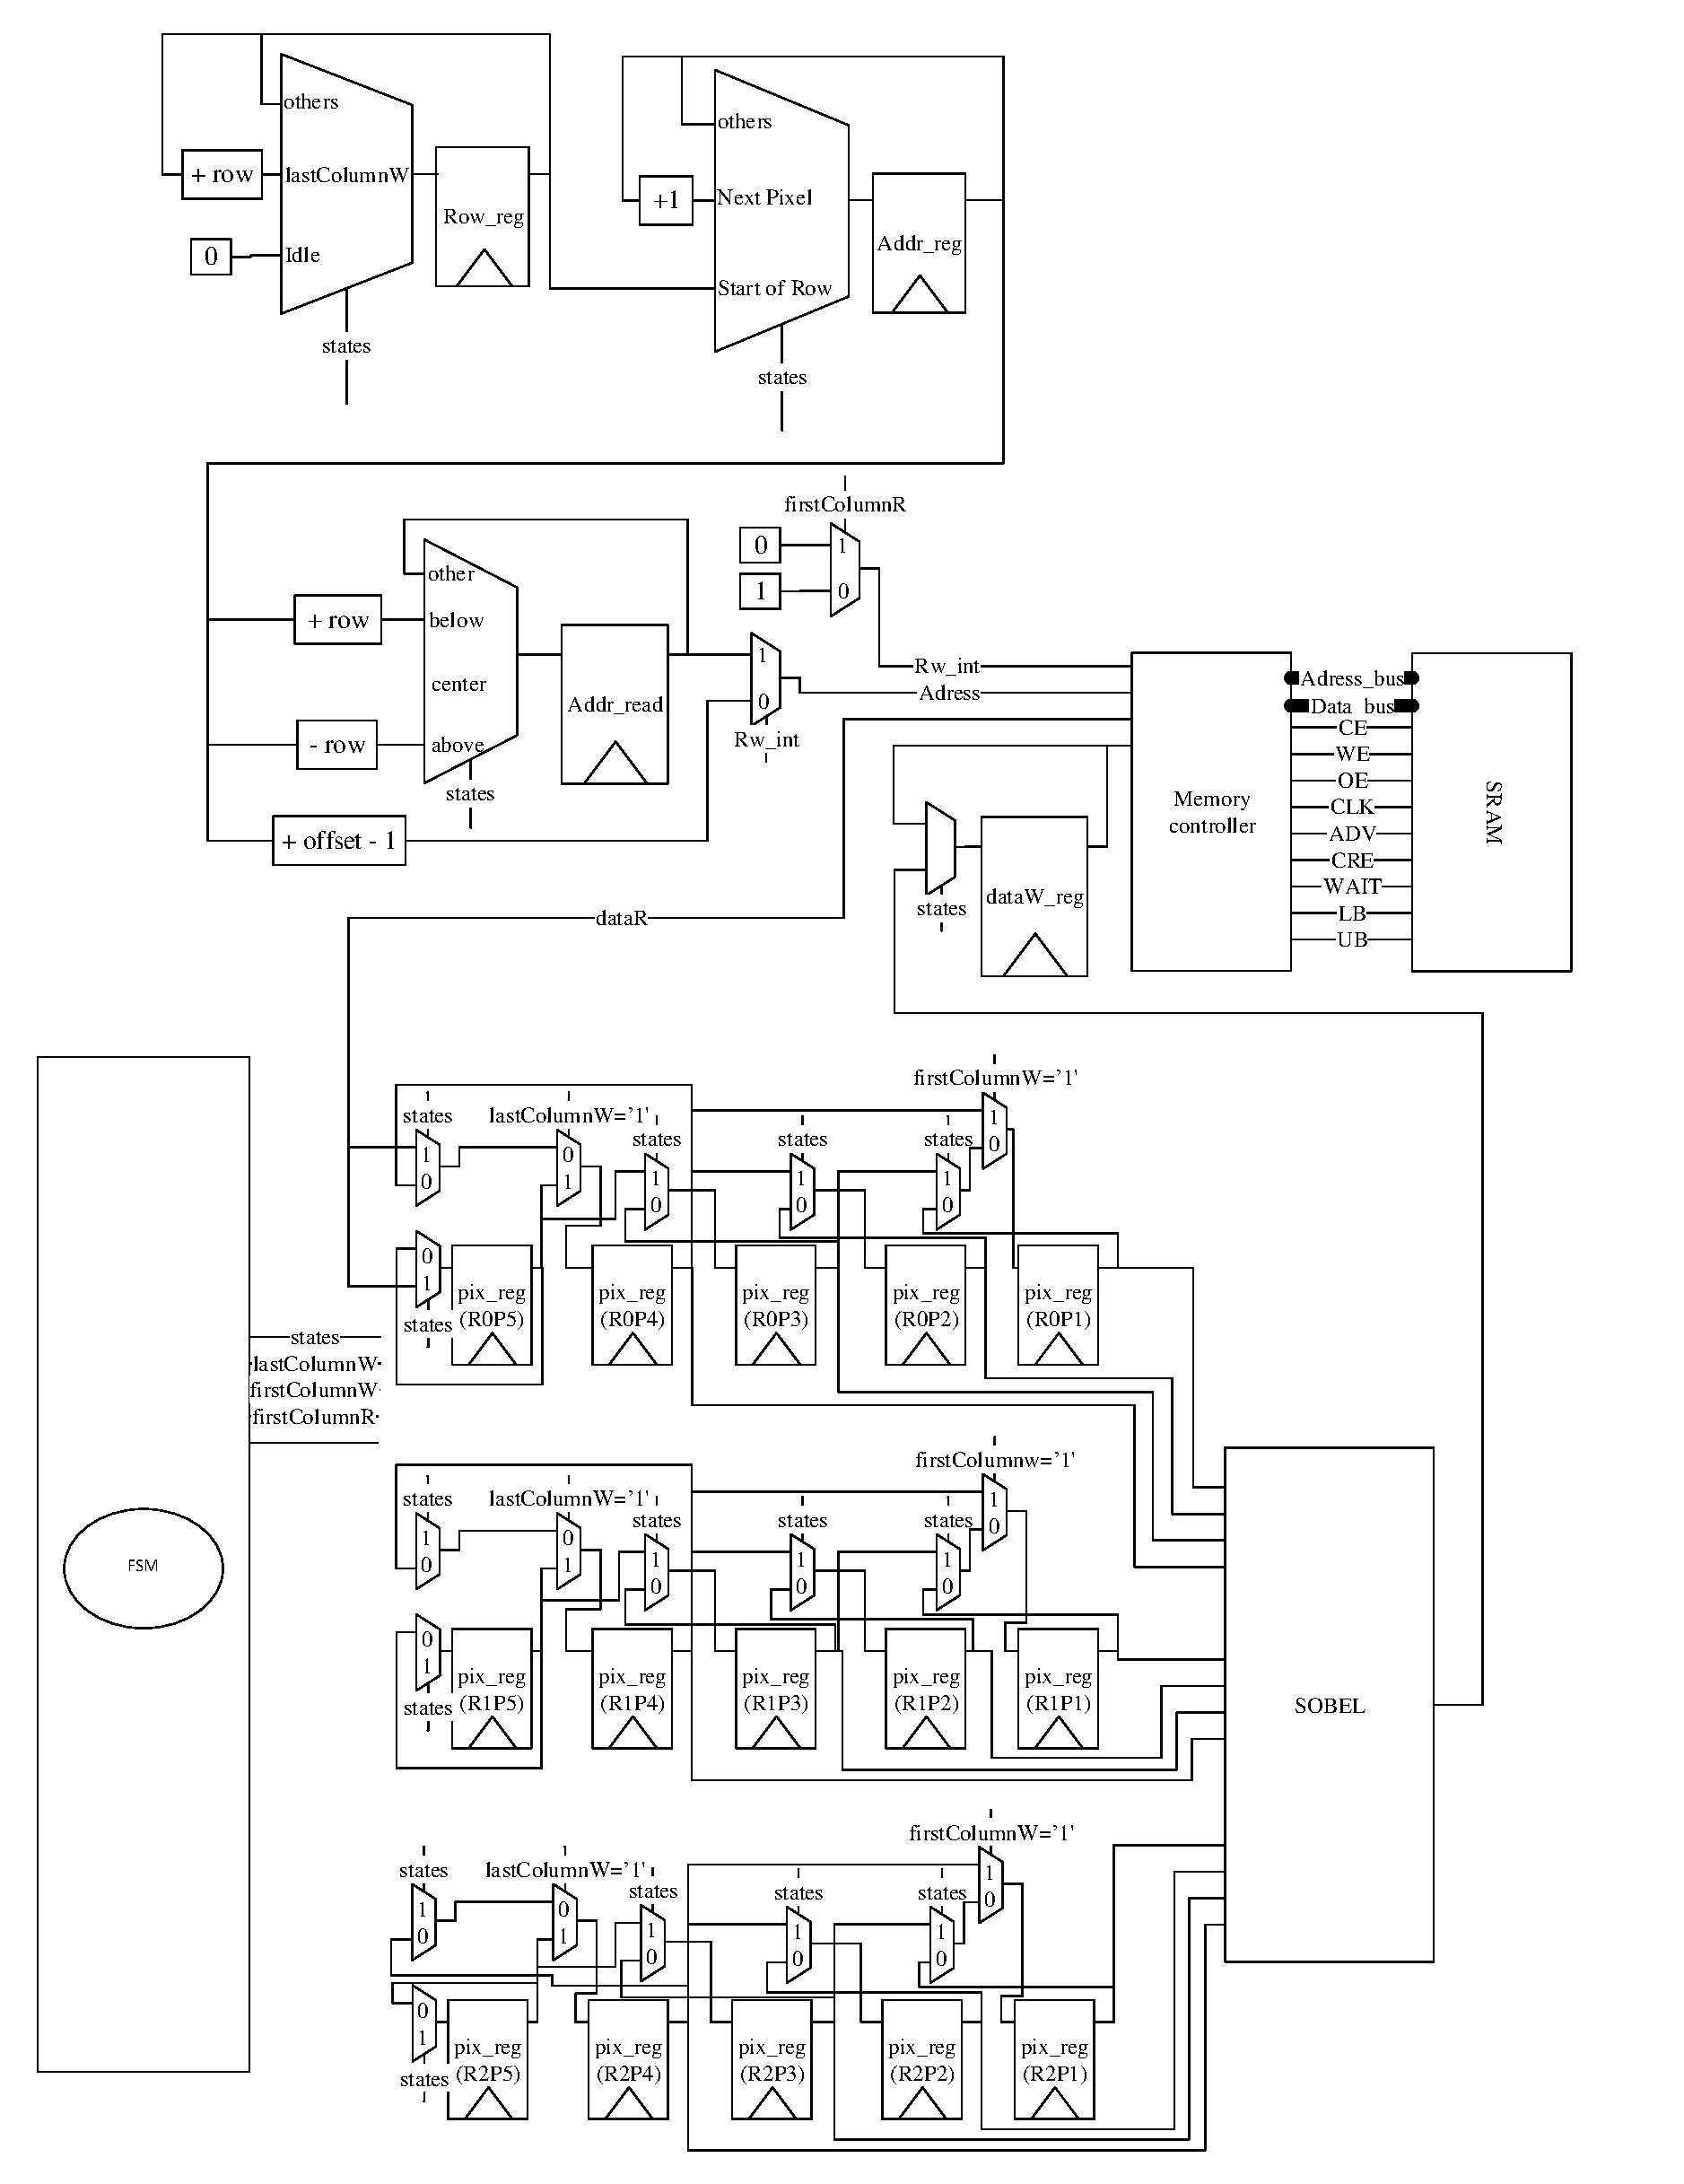
\includegraphics[width=1 \textwidth]{Block_diagram_detiled.pdf}
	\caption{Complete block diagram of the acc.vhdl code}
	\label{fig:block_acc}
\end{figure}